% Fix for: https://tex.stackexchange.com/a/315027/43228
\RequirePackage{luatex85}
\documentclass[border=10pt,17pt]{standalone}

\usepackage{cfr-lm}
\usepackage{pgf}
\usepackage{tikz}
\usetikzlibrary{arrows,shapes,decorations}
\usetikzlibrary{shapes.multipart}

\begin{document}

%% sans-serif fonts, large by default, and bold too
\sffamily
\sbweight
\bfseries
\large

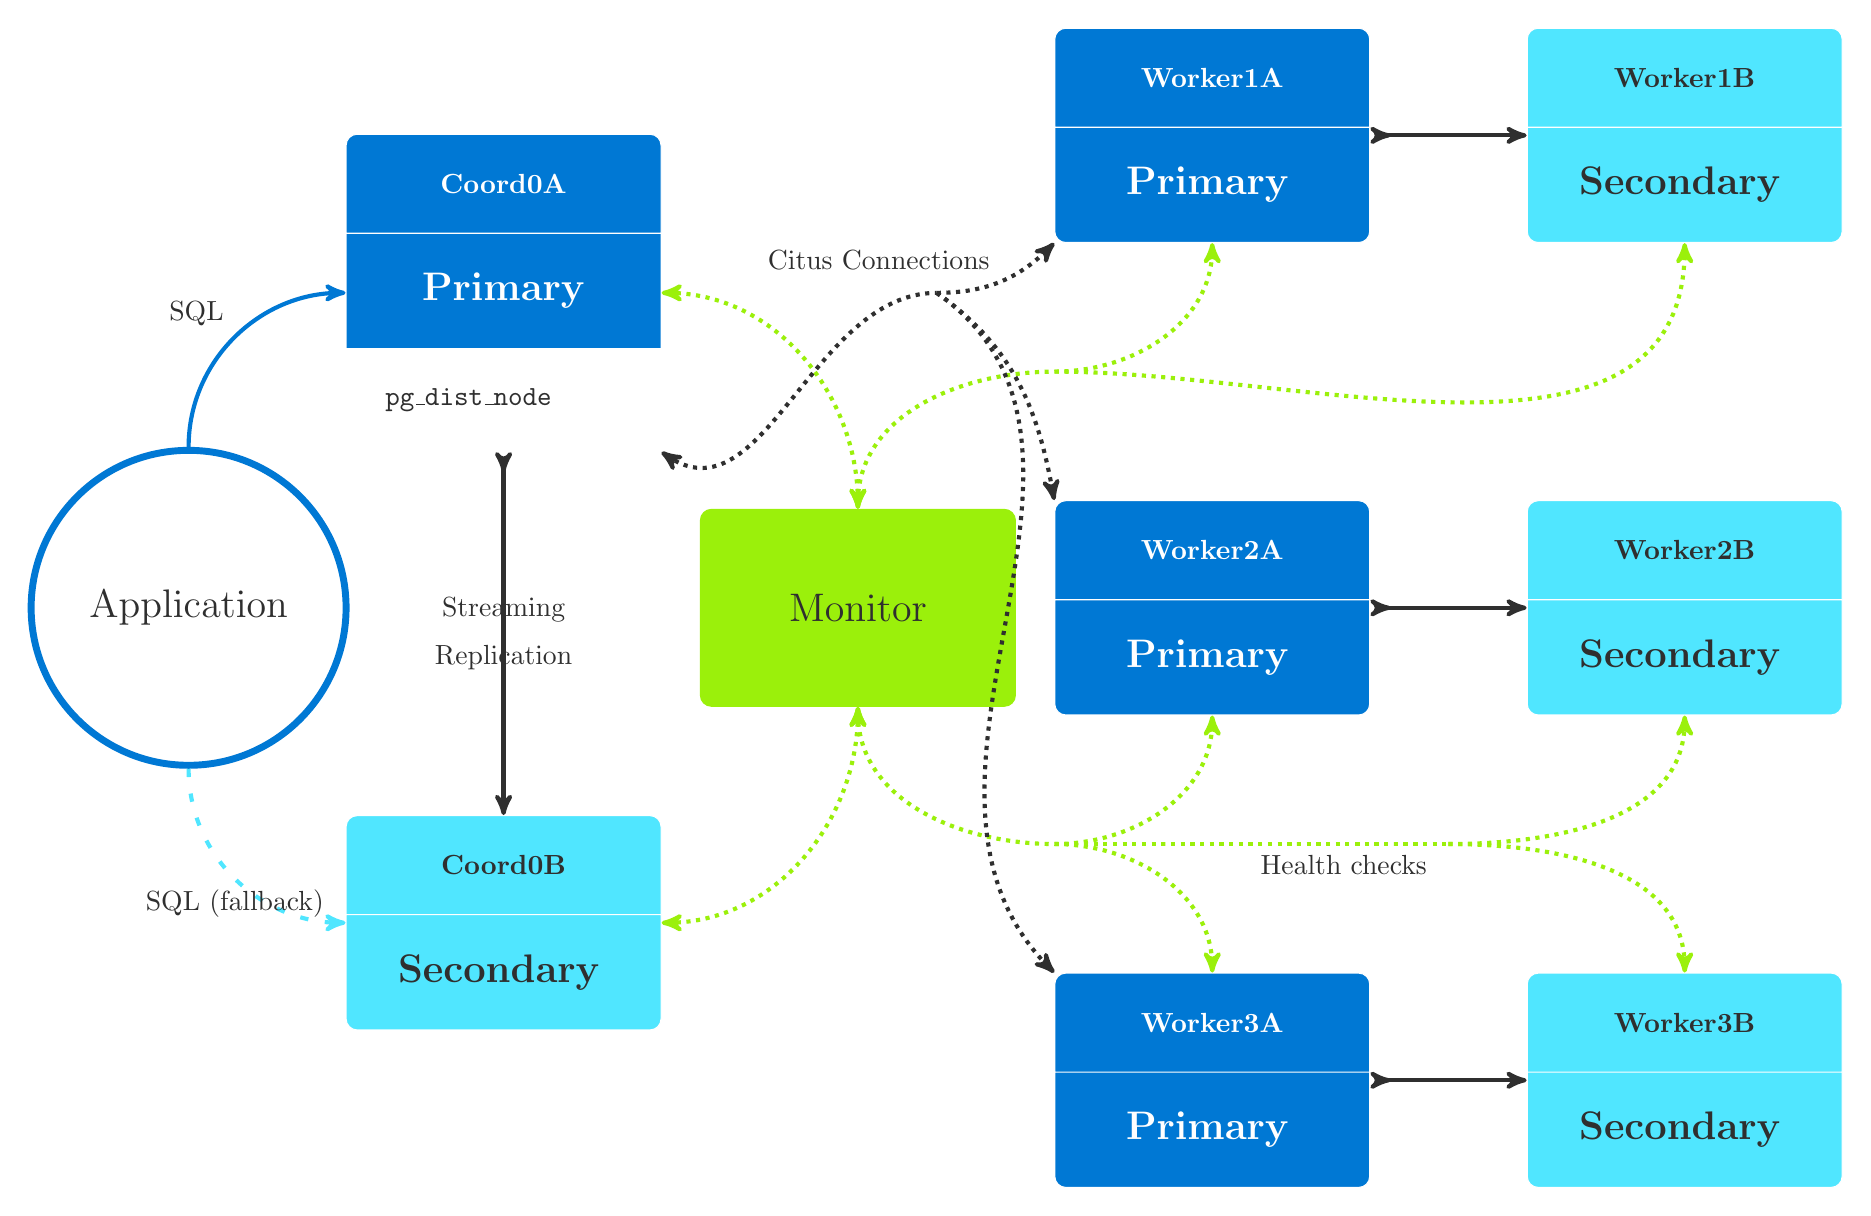
\begin{tikzpicture}[>=stealth',auto,rounded corners]

  \definecolor{pbox}{HTML}{0078D4} % MS blue
\definecolor{ptxt}{HTML}{FFFFFF} % white

\definecolor{sbox}{HTML}{50E6FF} % MS cyan
\definecolor{stxt}{HTML}{2F2F2F} % off-black

\definecolor{mbox}{HTML}{9BF00B} % MS light green
\definecolor{mtxt}{HTML}{2F2F2F} % off-black

\definecolor{apbox}{HTML}{0078D4} % MS blue
\definecolor{aptxt}{HTML}{2F2F2F} % off-black

\definecolor{async}{HTML}{EBEFF5} % very light grey

\tikzstyle{app}=[circle,thick,
	text=aptxt,draw=apbox,fill=white,
	line width=0.25em,minimum size=4cm]

\tikzstyle{node}=[rectangle,minimum height=2.5cm,minimum width=4cm]

\tikzstyle{mpnode}=[rectangle split,rectangle split parts=3,
	align=center,
	rectangle split part align={center, center, left},
	minimum height=2.5cm,minimum width=4cm,inner sep=0.5cm]

\tikzstyle{primary}=[mpnode,text=ptxt,draw=white,
  	rectangle split part fill={pbox,pbox,white}]

\tikzstyle{standby}=[mpnode,text=stxt,draw=white,
	rectangle split part fill={sbox,sbox,white}]

\tikzstyle{monitor}=[node,text=mtxt,draw=mbox,fill=mbox]

\tikzstyle{citusnode}=[rectangle split,rectangle split parts=2,
	align=center,
	rectangle split part align={center, center},
	minimum height=2.5cm,minimum width=4cm,inner sep=0.5cm]

\tikzstyle{cprimary}=[citusnode,text=ptxt,draw=white,
  	rectangle split part fill={pbox,pbox,white}]

\tikzstyle{cstandby}=[citusnode,text=stxt,draw=white,
	rectangle split part fill={sbox,sbox,white}]

\tikzstyle{sql}=[->,color=pbox,text=stxt,line width=0.15em]
\tikzstyle{sqlf}=[->,color=sbox,text=stxt,line width=0.15em,loosely dashed]
\tikzstyle{sr}=[>->,color=stxt,text=stxt,line width=0.15em]
\tikzstyle{hc}=[<->,color=mbox,text=mtxt,line width=0.15em,dotted]
\tikzstyle{hcmid}=[color=mbox,text=mtxt,line width=0.15em,dotted]
\tikzstyle{cw}=[<->,color=stxt,text=stxt,line width=0.15em,dotted]


  %% \draw [help lines] (-10,0) grid (10,20);

  \node  (c0a)   at (0,19)   [primary]
         {\textbf{\normalsize Coord0A}
           \nodepart{second}
           \textbf{\Large Primary}
           \nodepart[text=stxt]{third}
           \texttt{pg\_dist\_node}
         };

  \node  (c0b)   at (0,11)   [cstandby]
         {\textbf{\normalsize Coord0B}
           \nodepart{second}
           \textbf{\Large Secondary}
         };

  \node  (w1a)   at (9,21)  [cprimary]
         {\textbf{\normalsize Worker1A}
           \nodepart{second}
           \textbf{\Large Primary}
         };

  \node  (w1b)   at (15,21)  [cstandby]
         {\textbf{\normalsize Worker1B}
           \nodepart{second}
           \textbf{\Large Secondary}
         };

  \node  (w2a)   at (9,15)   [cprimary]
         {\textbf{\normalsize Worker2A}
           \nodepart{second}
           \textbf{\Large Primary}
         };

  \node  (w2b)   at (15,15)   [cstandby]
         {\textbf{\normalsize Worker2B}
           \nodepart{second}
           \textbf{\Large Secondary}
         };

  \node  (w3a)   at (9,9)   [cprimary]
         {\textbf{\normalsize Worker3A}
           \nodepart{second}
           \textbf{\Large Primary}
         };

  \node  (w3b)   at (15,9)   [cstandby]
         {\textbf{\normalsize Worker3B}
           \nodepart{second}
           \textbf{\Large Secondary}
         };

  \node  (app) at (-4,15)  [app]        {\Large Application};
  \node  (m)   at (4.5,15)   [monitor]    {\Large Monitor};

  \node  (midc) at (5.5,19)  [coordinate] {};

  \node  (mid1) at (7,18)  [coordinate] {};
  \node  (mid2) at (7,12)  [coordinate] {};
  \node  (mid3) at (12,12) [coordinate] {};

  \path (app) edge [sql,out=90,in=180]  node {SQL} (c0a)
              edge [sqlf,out=-90,in=180]  node[below] {SQL (fallback)} (c0b)

        (m)   edge [hc,out=90,in=0]  (c0a)
              edge [hc,out=-90,in=0] (c0b)
              edge [hc,<-,out=90,in=180] (mid1)
              edge [hc,<-,out=-90,in=180] (mid2)

        (mid1) edge [hc,->,out=0,in=-90] (w1a)
               edge [hc,->,out=0,in=-90] (w1b)

        (mid2) edge [hc,->,out=0,in=-90] (w2a)
               edge [hc,->,out=0,in=90]  (w3a)
               edge [hcmid,out=0,in=180] node[below,near end] {Health checks} (mid3)

        (mid3) edge [hc,->,out=0,in=-90] (w2b)
               edge [hc,->,out=0,in=90]  (w3b)

        (c0a) edge [sr] node[above] {Streaming} node[below] {Replication} (c0b)
        (w1a) edge [sr] (w1b)
        (w2a) edge [sr] (w2b)
        (w3a) edge [sr] (w3b)

        (c0a.south east) edge [cw,<-,out=-35,in=180] (midc)

        (midc) edge [cw,->,out=0,in=-135] node {Citus Connections}(w1a.south west)
               edge [cw,->,out=-35,in=100] (w2a.north west)
               edge [cw,->,out=-35,in=135] (w3a.north west);

\end{tikzpicture}

\end{document}
